% !TeX root = ../main.tex

\chapter{引言}

程序员问答网站是一种交互式在线问答社区。主流的程序员问答网站如StackOverflow保持着良好的社区活跃度,积累了大量讨论帖子。为了更好的讨论问题,提问者或回答者都会附上示例代码,即代码片段。这些代码片段围绕着提问者的问题编写,它们大多是局部的,无法编译的;代码片段能够帮助提问者和后来的问题浏览者,但它们可能无法保证安全性与高效性。智能合约是基于区块链的,它产生了与以往不同的安全性需求与高效性需求。本文研究的是程序员问答网站下智能合约代码片段的安全性与高效性。

本章首先对程序员问答网站、智能合约与代码克隆进行背景与意义介绍,然后再从程序员问答网站、智能合约与代码克隆三个角度阐述目前国内外相关研究,最后概括本文主要研究内容与贡献。其中,由于智能合约的出现以及相关研究内容与区块链高度相关,本文在智能合约的背景介绍章节介绍区块链。

\section{研究背景与意义}

程序员问答网站是编程人员重要的学习平台。如Abtahi等\cite{learnRust}的研究所示,程序员花费18\%的时间在如StackOverflow的程序员问答网站上提问与回答;36\%的时间学习官方示例。Allamanis等\cite{LDAso}的一项关于程序员问答网站如何帮助程序员的研究通过使用LDA(Latent Dirichlet Allocation)建模的方法,研究程序员问答网站帖子的讨论主题。StackOverflow的访问者集中讨论代码不生效、代码运行逻辑、如何实现功能、如何使用代码或API(Application Programming Interface),语言学习建议等主题。这些主题下的帖子可能有成千上百的访问量,同时高踞搜索引擎在相关问题的前列,这使得程序员问答网站的讨论广为人知,讨论中包含的代码片段也可能出现在各种软件系统中。

智能合约是一种新兴的区块链程序,它与一个虚拟账户绑定,这个账户储存着被称为以太币的虚拟货币。智能合约的每次运行被称作交易。完成交易需要被称为Gas的虚拟货币。随着智能合约的运行,以太币可能会交易到其他账户中。这让智能合约的安全性与高效性尤其重要;而基于区块链的运行环境又让程序员无法简单地套用过往的经验,这使得程序员更有可能编写糟糕的代码。

这为本文的研究提供背景,区块链以及它的一种脚本——智能合约是本文在程序员问答网站下的研究重点,相较于传统语言如C/C++、Java,智能合约的部署、运行环境与语言逻辑都有较大变化。本节下的前两小节将对本文的研究客体:程序员问答网站、智能合约进行介绍。最后一小节介绍本文方法依赖的关于代码克隆的背景知识。

\subsection{程序员问答网站}

在如今的软件工程领域当中,编程领域的快速发展为程序员带来了巨大的压力。面对技术挑战,开发人员经常求助于程序员问答 (Q\&A) 网站,例如 StackOverflow。在StackOverflow中,提问者以帖子的形式提出问题,这些帖子中存在的代码与文本形成了一个知识库。分析和理解这个知识库可以更好的帮助程序员使用程序员问答网站。本文的研究以StackOverflow为主。

首先,StackOverflow 上的提问者选择与他们的问题相关的标签(例如智能合约)进行发布。如图\ref{intro},他们可以在他们的帖子中附加图片、代码片段或链接,以帮助他们更好地描述想法。如果答案或问题描述不清楚,用户可以在问题或答案中添加评论,进行回复。当提问者认为一个答案解决了他的问题时,他也会将其标记为最佳答案。在这个过程中,代码片段经常是讨论的中心。提问者编写局部的、能够展示问题的代码片段并添加文本描述。回答者修改代码或重写一段新代码来解释他的答案。提问者和回答者编写的代码仅以表达想法为主,很少展示完整项目或者可编译代码文件。

\begin{figure*}[htbp]
\centering
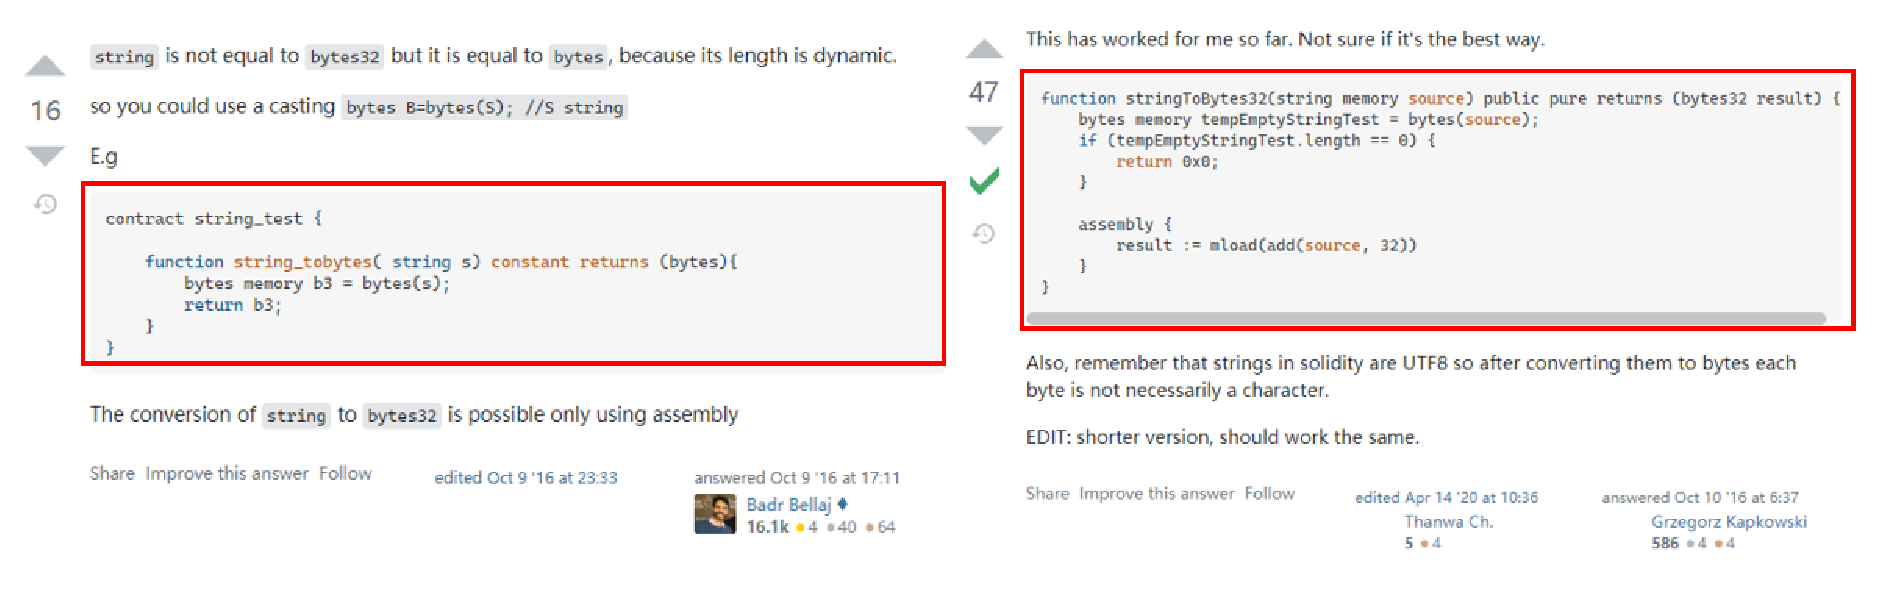
\includegraphics[width=0.98\textwidth]{figures/intro.eps}
\caption{来自StackOverflow的帖子示例}
\captionsetup{font={footnotesize}}
\label{intro}
%\vspace{-4mm}
\end{figure*}

程序员问答网站上出现的代码被称为代码片段(Code Snippet)。不完整的代码片段无法立即编译验证结果,一方面这不利于问题参与者进一步的讨论,另一方面这样的代码片段可能是存在漏洞或者低效率的,问题参与者与后来的问题浏览者可能错误的学习甚至复制了帖子的代码。

一种可能的情况是:程序员遇到代码无法运行等问题时,他们在StackOverflow上复制代码片段,并且直接在他们的项目中使用。这些未知的代码片段会给程序带来风险,因为在StackOverflow上功能满足程序员需求的代码片段不够完善,很少考虑如安全或效率问题,并非最佳实践。因此简单的复制可能存在缺陷。

Felix等的研究\cite{fisher1}表明,在StackOverflow上发布的1,161个有缺陷的Android代码片段被复制并粘贴到Google Play上可用的1,305,820个Android应用程序中。这些有缺陷的代码片段导致了实际项目中漏洞的严重传播。

\subsection{区块链与智能合约}

智能合约是一种运行在区块链上的脚本,本文主要研究以太坊下的智能合约。智能合约与它的运行环境,也就是区块链息息相关。
区块链的概念最早出现在中本聪 2008年的论文\cite{ASE69}中,它是比特币的底层数据结构。区块链依赖一种称为矿工的交易打包者,矿工将收集足够数量的交易信息,再将交易记录通过Merkle算法进一步散列,然后存储前一个区块的哈希,最终形成一个链接在前一个区块之后的新区块。区块链系统本身是分布式的,因为它将区块存储在持有数据的节点网络上。每个人都能够获得所有数据,这意味着所有的交易都是公开透明的。为了保证数据的一致性,所有节点都必须对数据达成共识,因此区块链系统最终通过使用非对称加密、工作量证明\cite{ASE69} 等技术,形成了一个不依赖第三方的价值转移网络。许多人认为,区块链将因其独特的安全性和可靠性\cite{ ASE83}而带来互联网的新变革。

比特币是去中心化加密货币的起点,它在五年的实践中验证了区块链技术的可行性与安全性。然而它的编程语言是图灵不完备的,它使用的是一种基于堆栈的脚本语言,这无法构建足够高级的应用。以太坊与智能合约的出现很大程度上解决了这个问题。

区块链平台以太坊在比特币的基础上引入了智能合约的概念,该术语由 Nick Szabo 等人\cite{smart_contract}在 1990 年代中期引入。

智能合约通常被视为在区块链系统上运行的代码脚本,并在满足预定义条件时自动运行。人们正在以太坊上开发多种类型的智能合约。用于开发智能合约的Solidity语言天生就是图灵完备的\cite{ASE84},开发者能够创建复杂的智能合约应用,包括但不限于金融交易、游戏、保险等。

智能合约与其他语言编写的程序类似,它的运行依赖以太坊区块链系统上某个地址下的代码(支持它的功能)与数据(保存它的状态)。智能合约与其他程序的不同之处在于它还是一种与虚拟货币有关的金融账户,智能合约编写者可以在智能合约存储虚拟货币,也就是以太币,并且通过编写代码的形式让交易可以自动化进行。智能合约一旦部署到以太坊公链上就无法删除,任何打包到区块的交易都是不可逆并且有迹可循的。

%智能合约漏洞
智能合约词源来自法律意义上的合约,智能的意思是可以在硬件和软件中嵌入多种合约条款(如留置权、担保、产权划分等),从而使合约违约对于破坏者来说代价高昂(如果需要,有时会令人望而却步)。这个逻辑在区块链层是正确的,因为在使用工作量证明作为共识机制的区块链系统中,仅当篡改者拥有超过区块链中51\%的算力时,才能够抢先完成一个更长的、伪造交易的链,这也就是知名的51\%攻击。然而智能合约是程序,由于程序编写者的疏忽与水平局限,程序本身可能产生各种各样的漏洞或者低效写法。这就可能导致事情的发展超乎想象。

例如导致以太坊分叉的The DAO攻击,The DAO(The Decentralized Autonomous Organization)是区块链公司Slock.it发起的一个众筹项目。The DAO项目通过发布自己的DAO代币的形式,总共筹到了超过1200万个以太币,几乎占到了当时以太币数量的14\%。然而他们的智能合约存在重大漏洞,黑客主要利用一种称为重入攻击的攻击盗取以太币。

\begin{figure*}[htbp]
\centering
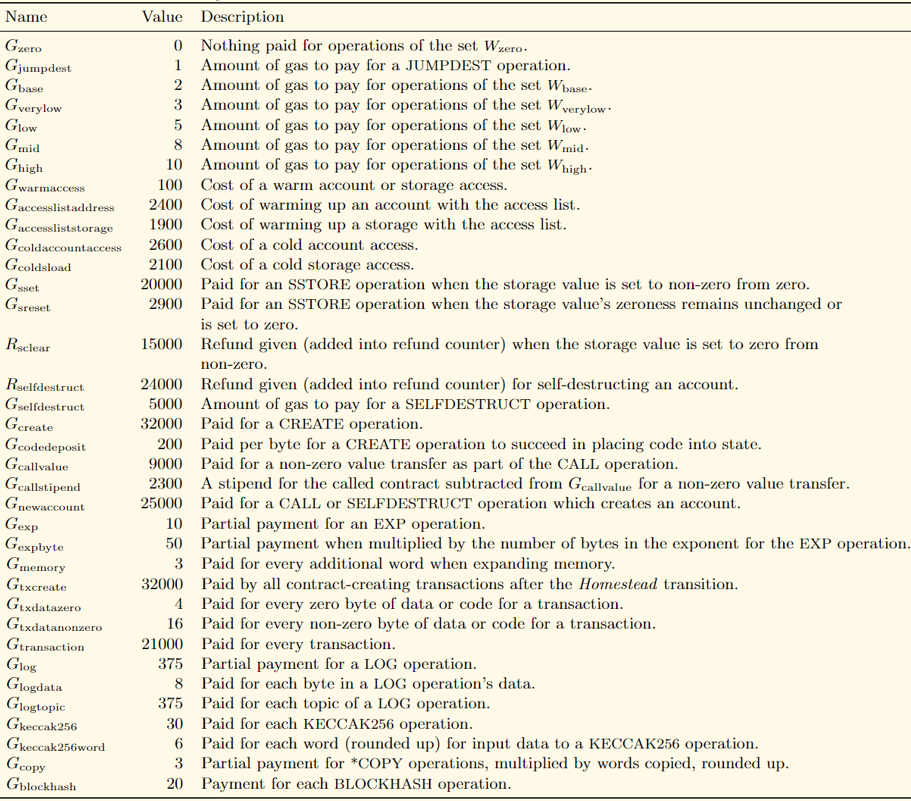
\includegraphics[width=0.8\textwidth]{figures/gasPrice.png}
\caption{字节码的Gas价格与描述}
\captionsetup{font={footnotesize}}
\label{gasPrice}
\end{figure*}

除了安全性的区别,以太坊应用了Gas这一概念。Gas是一种记账单位,它可以在EVM中计算交易费用,这涉及到以太坊依赖的区块链系统,交易费用是交易发送方支付给将交易打包到区块链中的矿工的以太币。对以太坊本身而言,执行操作需要花费一定计算与存储资源,而这些操作具体指的是智能合约经过编译后形成的字节码,字节码与其他语言编译后的机器码类似,是用于指挥计算机应做的操作和操作数地址的一组二进制数。字节码中的每一个二进制数都对应一定数量的Gas,当智能合约被调用时,EVM能够计算执行运行路径所需的字节码,所需的Gas就相应的被确定。

字节码的Gas消耗大致与计算机执行该字节码所花费的资源成正比。创建交易时,发送方必须指定 Gas 限额和 Gas 价格。 Gas 限额是发送者愿意在交易中使用的最大 Gas 量,Gas 价格是发送者希望支付给矿工的每单位 Gas 的 以太币数量。
这种做法的目的是激励矿工加速打包当前交易,Gas价格越高,矿工就越有动力将交易包含在他们的区块中,因此交易将更快地包含在区块链中。此时发送者在交易执行开始时预先购买全量 Gas(即 Gas 限额),并在交易结束时退还剩余 Gas。如果在任何时候交易没有足够的 Gas 来执行下一个操作,交易将被撤回,但发送者仍然为所使用的 Gas付费。这种费用机制旨在防范无意义合约的泛滥,防止合约执行过程中的无限循环,并更合理的分配网络资源。

就像用传统编程语言编写代码一样,程序员在编写智能合约时遇到问题合约可以到程序员问答网站(如StackOverflow)寻求帮助,因为程序员问答网站包含大量程序员分享的关于智能合约编程知识的帖子\cite{ASE61}。根据本文的统计,StackOverflow已有30,000多条带有智能合约标签的帖子,这说明在程序员问答网站,智能合约编程有相当的讨论度。对问答网站下智能合约的帖子的大规模研究有助于理解编程人员在什么方面存在错误实践,并且错误实践在现实环境中的扩散程度。

\subsection{代码克隆}

代码片段是软件系统的源代码文件中的程序代码的一部分。代码克隆的定义是在相同或不同软件系统中具有相同或相似代码的代码片段。这两个相似片段可能是来自于复制和粘贴操作,或者在一个原始片段对一些标识符和字符串进行了小的修改后,复制到其他软件系统。

不仅仅复制粘贴会导致代码克隆。代码克隆也可能来自于经常使用的代码模式,比如对应用程序接口 (API) 的调用(调用)可能需要特定的代码模式,而重复调用会创建相似的代码片段,这也是代码克隆。此外,来自自动源代码生成器的机器生成代码可以生成许多相同或相似的代码片段,它们也是代码克隆。本文所检测到的代码克隆以代码克隆对的形式存在。

在代码克隆领域,代码克隆对 (代码片段X, 代码片段Y)通常分为以下四种类型\cite{cloneIntro}。

\begin{itemize}

    \item[类型一] X 和 Y 是语法相同的代码片段,但可能存在非可执行元素(例如空格、制表符、注释等)的差异。
    
    \item[类型二] X 和 Y 是结构相同的代码片段,除了 类型一 的差异外,可能还有标识符名称、文字和类型名称的差异。分析克隆对中名称更改是发现代码克隆的重要方法。开发人员从原始部分复制代码片段并将其粘贴到不同的部分,并更改变量或类型以适应新的上下文。这种情况可以被检测为名称的不一致更改。
    
    \item[类型三] X 和 Y 是相似的代码片段,除了类型二的差异之外,可能因为语句添加、删除或修改到另一个片段产生差异。相关研究一般会根据它们设定的相似性结构给出一个相似阈值。较为复杂的相似性检测方法如检测两个字符或标记序列的编辑距离,或者从代码片段的特征值获得的两个向量的余弦值。
    
    \item[类型四] X 和 Y 在语法上是不同的代码片段,但它们的功能是相同的。
    
\end{itemize}

现有的方法用于找出相似代码的代码克隆对,可用于知识推荐,漏洞检测,代码异味寻找等领域。本文的目标是通过使用代码克隆找到漏洞与Gas低效模式定位一致的代码克隆对;本文的实践表明,相似度高的匹配对不意味着漏洞与低效模式定位一致。为了保证定位一致,本文根据语法一致、语义相似的原则,实现了本文的代码克隆方法。

\section{国内外研究现状}

本文的主要内容是使用代码克隆的方法解决了程序员问答网站领域下的有关智能合约语言的漏洞与Gas低效模式的检测问题。本节将从程序员问答网站行为分析与代码片段研究、基于智能合约的安全与Gas研究和代码克隆检测方法三方面介绍国内外的研究现状。

\subsection{问答网站实证研究与代码片段研究}

%近年来的有关研究主要分为帖子优化,代码重用,行为分析三个具体的子领域。
程序员问答网站如StackOverflow 包含大量的文本与源代码片段。目前该领域的大多数研究都集中在 StackOverflow 中帖子的文本和代码上。

StackOverflow的信息繁杂,帖子数量不断增长。全面了解StackOverflow的讨论主题变得更加困难。
一部分的研究关注于StackOverflow信息的收集与整理,通过实证研究的方式探究StackOverflow的热点问题、过时答案或代码缺陷等。

实证研究(Empirical Study)是指研究者亲自收集观察资料,为提出理论假设或检验理论假设而展开的研究。实证研究具有鲜明的直接经验特征。在StackOverflow的相关实证研究中,它们运用LDA等文本分析方法或者提取代码特征来获取数据,结果经验的分析来增强对StackOverflow的了解,寻找StackOverflow的运行规律。

Moses等\cite{analysis_modern} 发现现代软件公司在发布过程中出现了新的变化,如持续部署和基础设施,但开发人员和发布工程师觉得这些做法具有挑战性,并求助于 StackOverflow 等程序员问答网站来寻找答案。他们介绍了对 StackOverflow 中发布工程问题的实证研究结果,以了解现代发布工程的讨论主题及其难度。他们使用主题建模技术,发现 一方面,开发人员讨论了38个发布工程主题,涵盖了现代发布工程的所有六个阶段;主题合并冲突、分支和远程上游受到更广泛的讨论,而主题代码审查、Web 部署、MobileApp 调试和部署、持续部署讨论热度较低但更复杂。特别的,根据从 StackOverflow 收集的数据,发布工程主题“安全性”既广泛讨论又困难。
Baltes 等 \cite{so_torrent} 专注于 StackOverflow 上问答随时间的变化。  StackOverflow的问题和答案随着时间的推移而发展,例如,代码片段中的错误被修复,或是代码使用了更新的库,或者为了描述清晰而编辑代码片段周围的文本。他们构建了 SOTorrent以分析StackOverflow上的内容演变,这是一个基于官方数据转储的开放数据集。 SOTorrent 提供对整个帖子和单个文本或代码块级别的StackOverflow 内容的版本历史的访问。它通过聚合来自文本块的 URL 和收集从 GitHub 文件到StackOverflow帖子的引用,能够将StackOverflow帖子链接到其他平台。

Zhang等 \cite{obsolete_answer} 关注过时的答案,他们发现如果没有明确识别或记录,过时答案可能会误导寻求答案的人并导致意外问题(例如,使用过时的安全协议)。他们调查了答案中的知识是如何变得过时的,并确定了这些过时答案的特征。最终发现:1) 超过一半的过时答案 (58.4\%) 在首次发布时可能已经过时。 2)当观察到一个过时的答案时,只有一小部分(20.5\%)的答案会被更新。 3) 某些标签(例如,node.js、ajax、android 和 Objective-c)中的问题的答案更有可能过时。研究结果表明,Stack Overflow 应该开发机制来鼓励整个社区维护答案(以避免过时的答案),并鼓励寻求答案的人仔细阅读答案中的所有信息(例如评论)。Diamantopoulos等 \cite{data1} 提出了一种方法,允许在 StackOverflow 中搜索解决方案,他们通过帖子的主要元素的相似检索解决问题,这些主要元素不仅包括标题、标签和正文,还包括源代码片段。他们介绍了这些元素的相似性检索方案,并实现从源代码片段中提取结构信息进行比较的检索方式。评估结果表明,这个方法在推荐相似帖子上是有效的,允许StackOverflow用户在不完全提供问题信息的情况下进行搜索。

Keivanloo等 \cite{data2} 发现代码搜索引擎不能成功地找到工作代码示例。代码搜索引擎未能将高质量的代码示例排在结果的顶部。同时,由于时间复杂度高或查询语言限制,已有解决方案无法直接集成到大规模的源代码引擎中。他们提出了一种发现工作代码示例的方法,该方法可以被大规模的源代码搜索引擎采用。这个方法的时间复杂度与互联网 上现有代码搜索引擎的复杂度一样低,并且该时间复杂度大大低于支持自由格式查询的基于模式的方法。Park 等 \cite{data3} 研究如何即时检索代码以供参考。检索代码的传统模式一直将代码视为文本并通过关键字搜索技术解决问题。这种方法的局限性:(1)代码的语义描述仅限于注释。(2)句法关键字通常没有足够的选择性。他们通过为提交到存储库的代码添加语义标签来增强基于关键字的语义方法。具体的,他们在代码的抽象向量上提出了可扩展的索引结构。他们将这个技术部署到即时搜索和标记场景:对于即时代码搜索场景,实现了一个即时克隆搜索工具,支持超过 5400 万个 
定位的亚秒级搜索。对于即时代码标记场景,提出了一种自动即时代码标记算法来从克隆中挖掘有意义的标签。

StackOverflow上的学习者往往会发现能够解答他们问题的帖子答案中的代码片段是可用的,只需要简单的复制粘贴或者稍微改动部分代码,就能将代码片段转移到他们的项目当中;对于这些帖子的代码片段的安全性与代码片段的转移导致漏洞的扩散问题,在StackOverflow上的安全方向,也有相应研究。

Fischer 等人的一项研究\cite{fisher1} 使用深度学习来查找不安全的代码片段,并发现在130 万个 Android 应用程序中,有15.4\%的应用程序包含来自StackOverflow的代码片段。7.9\%的应用程序至少包含一个不安全的代码片段。Fischer 等 \cite{fischer2} 在进一步的研究中,发现生产环境的代码受到 Stack Overflow 上给出的示例的启发,通过复制和粘贴功能代码,开发人员将可被利用的软件漏洞引入每天由数百万用户安装的应用程序中。这指出本文要在不安全代码到达剪贴板之前,直接在StackOverflow与不安全代码作斗争。他们的工作专注于通过应用助推(从行为科学中借用的概念)来支持软件开发人员做出更好的决策。他们的一个主要发现是:对于 Stack Overflow 上 99.37\% 的不安全代码示例,可以使用类似的替代方案来服务于相同的用例并提供更强大的密码学相关代码。他们的系统设计基于由深度神经网络。这个系统学习了加密 API 使用模式的表示及其安全性分类。实验证明了基于助推的安全建议有助于解决 Android 中最流行和最容易出错的加密用例。

%Stolee 等 \cite{data5} 发现纯文本无法捕捉代码片段的语法结构;例如,片段经常引用特定的Android API,但由于以往方法将片段视为文本,Android API的特殊性 并不总是显而易见的。他们执行片段分析以从 Stack Overflow 中常见的短纯文本片段中提取结构信息。该分析能够从 21,250 个 Stack Overflow 代码片段中识别出 253,137个方法调用和类型引用,实验证明了当前方法在实践中比基于代码块的词法搜索执行得更好。

Hyunji等\cite{dicos}展示了 Dicos,这是一种通过检查 Stack Overflow 帖子的更改历史来发现不安全代码片段的准确方法。当在帖子中检测到安全问题时,用户讨论会将不安全的代码修复为安全,并且留下更改历史记录。受此过程的启发,Dicos 首先从 Stack Overflow 帖子中提取更改历史记录,然后利用可有效识别安全补丁的预选特征分析帖子历史是否包含安全补丁。最后,当检测到此类更改时,Dicos 会确定在应用安全补丁之前的代码片段是不安全的。为了评估 Dicos,他们收集了 1,958,283 篇带有 C、C++ 和 Android 标记的 Stack Overflow 帖子。当他们对收集的帖子应用 Dicos 时,Dicos 从收集的帖子中发现了 12,458 个不安全的帖子(即 14,719 个不安全的代码片段),这个方法的准确率为 91\%,召回率为 93\%。他们进一步证实,在 2,000 个流行的 C/C++ 开源软件中,有 151 个的最新版本包含至少一个取自 Stack Overflow 的不安全代码片段。

以上的工作从寻找热点问题与代码片段安全的角度进行研究。与本文的工作相比,以上工作大多基于C/C++、Java等传统语言,而少有针对程序员问答网站下智能合约的研究。这是因为传统语言的基础工具链相当丰富,在智能合约领域下尚且没有足够的基础工具,这也使得本文转用代码克隆方法进行研究。智能合约的安全漏洞与低效模式也与传统语言有较大不同,这使得本文在这部分的处理与现有研究不同。

\subsection{基于智能合约的安全与Gas研究}

以太坊是目前较为流行的加密货币。本文的研究与以下列出的研究以以太坊为研究对象。目前,已有数万份智能合约运行在以太坊。

漏洞检测的相关研究通常会提供漏洞检测的工具,这些检测方法大多基于符号执行,通过输入完整源代码或者字节码,可以获取代码上的漏洞信息。

Luu等 \cite{oyente}发现了能够被他人操纵获利的智能合约漏洞。为了帮助编写合约的开发人员,他们构建了一个名为 Oyente 的符号执行工具。实验表明,在 19,336 份现有的以太坊合约中,Oyente 将其中 8,833 份标记为易受攻击,包括在 2016 年 6 月导致 6,000 万美元损失的 The DAO 漏洞。在Oyente的基础上存在很多工作 \cite{honey}\cite{Osiris}\cite{maian}。Torres等 \cite{honey} 发现一种更隐蔽的攻击方法正在兴起。攻击者不再搜索易受攻击的合约;相反,他们试图通过部署包含隐藏陷阱的看似易受攻击的合约来引诱受害者进入陷阱。这种新型合约通常被称为蜜罐,他们首次对蜜罐智能合约进行了系统分析。开发了蜜罐技术的分类法,并使用它来构建 HoneyBadger——一种使用符号执行的启发式工具。论文对超过 200 万份智能合约进行了大规模分析,结果表明工具准确率与运行效率高。他们最终在以太坊识别出 690 个蜜罐智能合约和 240 个受害者,发现蜜罐创建者累计获利超过 90,000 美元。于实验准确率方面,人工验证表明,87\% 的报告合约确实是蜜罐。
Torres等 \cite{Osiris} 关注与算术错误相关的漏洞,由于以太坊虚拟机和 Solidity 编程语言特性,这类错误特别难以避免。他们介绍了 Osiris——一个结合了符号执行和污点分析的工具,以便准确地发现以太坊智能合约中的算术错误。论文在一个包含超过 120 万个智能合约的大型实验数据集上评估了它的性能,发现 42,108 个合约包含算术错误。

Nikolic等\cite{maian}提出了一类称为跟踪漏洞的新型漏洞。此类跟踪漏洞总共两种:资金锁死或自杀合约,实现了 Maian,这是第一个用于发现跟踪漏洞的工具,它采用过程间符号分析和具体验证器来发现漏洞。论文对近一百万份合约进行分析,在抽样用于具体验证和手动分析的 3,759 份合约的子集上,以 89\% 的真阳性率重现真实漏洞的触发,发现 3,686 份合约的漏洞触发。这个工具发现了臭名昭著的 Parity 漏洞,该漏洞间接锁死了价值 2 亿美元的以太币。Durieux等\cite{tool_paper}使用两个新数据集对9种最先进的自动分析工具进行了实证评估,使用了两种数据集:分别是69个带注释的可用于评估分析工具的精度的易受攻击智能合约的数据集与包含以太坊区块链中开源智能合约的数据集。这些智能合约在 Etherscan 上具有 Solidity源代码(总共47,518个合约)。SmartBugs旨在多种分析工具之间的集成和比较。实验上,他们使用 SmartBugs对两个数据集执行9个自动分析工具。总共进行了 428,337 次分析,耗时约564天零3小时,无论是工具数量还是执行时间,都是迄今为止最多的。实验发现,所有工具仅检测到数据集中42\%的漏洞,其中Mythril工具具有更高的准确度(27\%)。他们观察到 97\%的合约被标记为易受攻击,因此表明存在大量误报。实际上,针对同一份代码,四个或更多工具同时检测到的漏洞数量很少。

Gas相关研究与漏洞类似,以工具的形式对数据进行检测,但Gas是一次运行下用于打包交易的虚拟货币,如果没有本次运行的输入,那么将无从估计Gas消耗;因此Gas相关研究从提取Gas低效模式入手。

Chen等\cite{saveMoney}对优化不足的智能合约进行了首次深入调查。他们首先从真实智能合约的执行痕迹中识别出 24 种模式。然后,他们设计和开发了GasReducer,这是第一个从智能合约的字节码中自动检测漏洞并通过字节码优化,使用高效代码替换旧代码的工具。通过使用 GasReducer 分析所有智能合约及其执行轨迹,他们分别在部署和调用智能合约时检测到 9,490,768 和 557,565,754 个漏洞实例。

Kong等\cite{gasPattern}发现由于开发人员不熟悉智能合约(即以太坊虚拟机)的操作环境,或者在开发过程中不注意资源消耗,因此智能合约有很多优化空间。为了填补这一空白,他们从超过25,000篇帖子中定义了6个气体低效率的模式,并提出了一种源代码级别的优化方法。为了评估Gas低效模式的频繁程度和可能造成的经济损失,他们对超过16万份真实的智能合约进行了实证研究。实验结果表明,52.75\%的合约中至少含有一种Gas低效模式。如果从合约中删除这些模式,每个合约至少可以节省0.30美元。

Chen等\cite{GasChecker}总结了十种Gas效率低下的编程模式,并提出了一种基于SE(symbolic Execution)的新方法,开发了名为 GasChecker 的工具。GasChecker在智能合约的字节码中检测Gas低效模式。为了使他们的方法可扩展以分析数百万个智能合约,他们通过将 SE修改为 MapReduce 编程模型来并行化运行SE,并提出一种新的基于反馈的负载平衡策略以有效利用云资源。大量实验表明,GasChecker 可以随着云节点的增加而很好地扩展。许多开源智能合约包含各种低效的代码。人工调查表明,只有 2.5\% 的已发现Gas低效模式实例是误报。

%Chen等人 \cite{define_defect} 从以太坊 StackExchange 以及现实世界的智能合约中收集了与智能合约相关的帖子。他们手动分析了这些帖子,使用它们来定义 20 种合约缺陷。他们将它们分类为潜在安全性、可用性、性能、可维护性和可重用性问题。为了验证从业者是否认为这些合约有害,他们创建了一项在线调查,并收到了来自 32 个不同国家的 138 份回复。反馈显示从业者认为这些合约缺陷是有害的,消除它们将提高智能合约的质量和稳健性。他们在 587 个现实世界的智能合约中手动识别了他们定义的合约缺陷,并公开发布了这份结果。最后,他们总结了合约缺陷造成的 5 种影响。这些有助于开发人员更好地了解缺陷的症状和修改优先级。

%He等 \cite{clone_esystem} 提出了第一个大规模的系统研究来描述以太坊智能合约生态系统中的代码重用实践。他们首先对他们获得的 1000 万份合约的数据集进行了详细的相似性比较研究,然后他们进一步进行了定性分析,以了解代码重用与漏洞之间的相关性,并且检测抄袭 DApp的数量。他们的分析显示,超过 96\% 的合约有重复,这表明生态系统高度同质化。他们的结果还表明,大约 9.7\% 的相似合约对具有完全相同的漏洞,他们假设这些漏洞是由代码克隆引入的。此外,他们确定了 41 个 DApp 集群,涉及 73 个抄袭 DApp,占原始市场量的 1/3。这给原创者造成了巨大的经济损失。

%Gao等 \cite{smartembed} 提出了一个名为 SMARTEMBED 的 Web 服务工具,它可以帮助 Solidity 开发人员找到智能合约中重复的合约代码和克隆相关的错误。他们的工具基于代码嵌入和相似性检查技术。通过比较以太坊区块链中现有Solidity代码的代码嵌入向量与已知bug的相似性,他们能够有效识别用户提供的任何Solidity代码的代码克隆和克隆相关的bug,有助于提高用户的安全性。除了供个人开发者使用外,SMARTEMBED还可以大规模应用于智能合约的研究。当应用到从以太坊区块链收集的超过 22K 的 Solidity 合约时,他们发现 Solidity 代码的克隆率接近 90\%,远高于传统软件,基于他们的算法可以高效准确地识别出 194 个克隆相关的 bug。精度为 96\%。

在这些工具中,漏洞检测方面,不同的工具有着不同的检测范围与检测逻辑,但它们的一个共性是无法应用在程序员问答网站上的代码片段上,这是由于代码片段是局部的、无法编译的;而本文的方法解决的就是这个问题。在Gas检测方面,相较于漏洞检测,工具数量与热度稍逊,但寻找Gas低效模式的逻辑却与漏洞接近,因此也可以用到本文的方法中。

\subsection{代码克隆检测方法}

对源代码,既可以理解为文本进行文本处理,也可以理解为代码,提取中间表示。根据对源代码的解析方式不同,代码克隆技术主要有: 基于文本(Textual)的技
术,基于词块(Token)的技术,基于语法(Syntactic)的技术,基于语义(Semantic)
的技术。

基于文本的技术比较两个代码片段,如果这两个代码片段在文本内容方面字面上完全相同,则将它们声明为克隆。基于文本的克隆检测技术产生更少的假阳性,易于实现且与语言无关。

Roy等\cite{nicad}开发了一种基于文本的代码克隆检测技术,称为NICAD (Accurate Detection of Near-miss Intentional Clones)。NICAD工具\cite{clone13}使用两种克隆检测技术:基于文本和基于抽象语法树的克隆检测技术,以检测类型一、类型二和类型三的克隆代码。这两种方法相互补充,克服了技术本身的局限性。NICAD有三个阶段。1)解析器提取函数并切段,将语句的不同片段分解成行。2)将语句的片段规范化,以使用转换规则忽略编辑差异。3)使用动态聚类来检查潜在克隆的重命名、筛选或抽象,以便对潜在克隆进行简单的文本比较。他们采用最长公共子序列(LCS,Longest Common Subsequence)算法,一次性比较文本与抽象语法树的克隆。这一系列处理使得每个潜在的文本克隆都必须与抽象语法树的克隆进行比较,比较成本很高。

Jeong等\cite{sdd}使用了一种基于文本的代码克隆检测技术Sdd。Sdd能够高性能检测重复的代码。它通过使用反向索引\cite{clone57}和使用n邻域距离算法\cite{clone57}的索引数据结构来检测精确和相似的代码克隆;但这些处理导致它的假阳性较高。

基于文本的技术\cite{clone4}\cite{clone8}\cite{clone10}有如下局限性。1)不能用逐行的方法处理标识符重命名。2)带有换行符的代码片段不会被检测为克隆。3)当比较代码的两个片段,其中一个片段有方括号,另两个片段没有方括号时,添加或删除可能会产生方括号。

Ducasse等\cite{Ducasse}通过额外增加了过滤步骤,在克隆代码中提取有用信息,如间隙大小。间隙大小可以说明一个克隆对之间的非重复子序列的长度。例如,如果比较行序列“abcghdjgi”和“abcfklngi”,则间隙长度为4,因为两个非重复子序列ghdj和fkln的长度为4。这有助于去除噪声和过滤,可以避免假阳性。过滤步骤使用了两个指标。1)最小长度:它是一个序列对中的最小长度。2)最大间隙大小:序列通过复制粘贴产生的最大间隙大小。Ducasse的工具还使用词汇分析来删除代码中的注释和空白,并使用动态模式匹配算法找到克隆。该工具的输出是代码克隆对的数行。它使用针对字符串的哈希函数来划分行,以获得更快的性能。Koschke\cite{Koschke}证明Duploc只检测到完全相同的复制粘贴的片段。它不能检测类型3的克隆,或处理复制粘贴代码中的修改和插入。Duploc无法检测复制粘贴的bug,因为检测bug需要语义信息,而Duploc只检测语法克隆。

词汇方法也被称为基于标记的克隆检测技术。在编译器的词法分析阶段,所有的源代码行都被划分为一个标记序列,然后匹配标记序列行。

Kamiya等人\cite{clone4}开发了一种称为CCFinder(Code Clone Finder)的后缀树匹配算法。CCFinder有四个阶段。1)词汇分析器从标记序列中删除标记之间的所有空白。2)使用转换规则转换标记序列。执行参数替换,将每个标识符都被一个特殊的Token替换。3)匹配检测阶段检测等效对作为克隆,并使用后缀树匹配识别克隆的类别。4)将克隆对的位置转换为原始源文件中的行号。CCFinder应用了几个度量标准来检测克隆。这些指标为:1)代码片段的长度:CCFinder用标记的数量或代码片段的行数来确定。2)克隆类的种群大小:克隆类中的元素的数量。3)标记的数量和克隆类中元素的数量的组合:可以用于估计重构代码大小。4)代码克隆覆盖率:任何克隆的行或文件的百分比。它还优化了算法,以降低标记匹配算法的复杂性。

Li等\cite{clone8}\cite{clone35}使用一种基于Token的技术来检测与大型软件系统中的错误相关的代码克隆。他们的工具CP-Miner(Clone Pair Miner)使用频繁的子序列挖掘\cite{clone24}来查找复制粘贴的代码块。CP-Miner通过解析源代码来构建一个包含序列集合的数据库,将这个问题转换为一个子序列挖掘问题。他们还实现了CloSpan算法\cite{clone24}的一个增强版本,用于满足子序列中的间隙约束。这个方法下,每个相似的语句与每个函数名都被映射到相同的标记。

Kamiya等\cite{clone65}开发了一种基于标记的技术FRISC,它将每个重复的指令转换为一种特殊的形式,并使用后缀数组算法来检测克隆。FRISC有五个步骤。1)进行词法分析和规范化,将源文件转换为Token序列,并用特殊的Token替换每个标识符。2)生成语句哈希值,它为“;”、“\{”和“\}”之间的每个语句生成一个哈希值,其中每个Token都包含在一个语句中。3)折叠重复指令,识别每个重复的子序列,接着删除重复的子序列,并保存它们的重复次数。4)检测相同的哈希子序列,从折叠的哈希序列中检测相同的子序列。如果标记数量的和小于最小标记长度,则不被认为是克隆。5)将相同的子序列映射到源代码,从而将克隆对转换为源代码。

语法方法可分为两种技术。这两类分别是基于树的技术和基于度量的技术。基于树的技术使用解析器将源代码解析为一个抽象语法树(AST,Abstract Syntax Tree),并对子树进行比较,以使用树匹配算法找到克隆的代码。

Baxter等人\cite{clone13}实现一种基于树的代码克隆检测技术CloneDr。它可以检测精确克隆、相似克隆和AST重构。在将源代码解析为AST后,它通过应用三种主要算法来找到克隆。第一种算法检测子树克隆,第二种算法检测可变大小的子树克隆序列,如声明或语句序列,第三种算法通过使用其他克隆组合来发现更复杂的遗漏的克隆。该方法使用哈希函数分割子树,然后比较同一个桶中的子树。当第一个算法找到子树克隆,会将每个子树与其他子树进行比较。

Wahler等人\cite{clone34}通过应用频繁项集挖掘来检测在XML中以抽象语法树(AST)表示的克隆。频繁项集挖掘用于查找频繁发生的动作或事件序列。一个实例被称为事务,每个事务都有许多被称为项的特性。该工作使用先验算法\cite{clone52}来识别大量数据中的特征。

在基于度量的克隆检测技术中,通过比较度量,而不是直接比较代码,来计算每个代码片段或AST,以找到相似的片段。

Kodhai等人\cite{clone19}将基于度量的方法与基于文本的方法结合起来,以检测C语言中的函数克隆。克隆检测的过程分为五个阶段。1)分析文件以删除预处理器语句、注释和空格。源代码被重建为一个标准形式,便于检测克隆片段的相似性。2)进行潜在克隆的文本比较。它会重命名数据类型、变量和函数名称。3)对每种函数进行识别并进行提取。4)度量计算。5)针对类型一和类型二的克隆检测。基于文本的方法发现克隆具有较高的准确性和可靠性,但基于度量的方法可以通过使用计算的度量值来降低基于文本的方法的高复杂性。这种方法的局限性是,它只检测类型一和类型二克隆,具有较高的时间复杂度。

Abdul等人\cite{clone48}基于度量的使用了一种分形聚类算法。这种技术需要四个步骤。1)对输入的源文件进行预处理。2)提取所有片段。3)利用分形聚类方法将片段集划分为三种类型的少量聚类。主要集群覆盖类型一和类型二克隆,中间集群覆盖类型一和类型三克隆,而一个单例集群则不认为是克隆。4)从主集群中提取克隆类。

Horwitz等\cite{clone22}使用程序切片\cite{clone38}来寻找同构的代码依赖图PDG子图和代码克隆。切片克隆检测算法执行三个步骤。1)通过将所有PDG节点划分为等价类来找到克隆对,其中同一类中的任何两个节点都是匹配的节点。2)删除已包含的克隆对。当且仅当该克隆对中的每个元素都是另一个克隆对中的另一个元素的子集时,一个克隆对才包含另一个克隆对。因此,需要删除所包含的克隆对。3)利用传递闭包合并克隆对形成更大的组。

%Krinke等\cite{clone22}通过寻找具有高精度和查全率的最大相似PDG子图检测克隆。PDG包含表示表达式的顶点和边。它还包含依赖关系边。值依赖关系边表示表达式之间的数据调用。另一条边,也就是引用依赖关系边,表示对变量的赋值。

%与这些工作不同,我们重点分析来自 StackOverflow 的Solidity 代码。我们还使用诸如 Oyente 之类的错误检测工具来定位错误。我们的方法实现了对来自 StackOverflow 的智能代码的错误识别的自动过程。
与这些工作不同,本文的方法基于抽象语法树,获得语法一致而语义相似的代码克隆对,这是由于需求不同。本文用代码克隆方法找到程序员问答网站代码片段上的漏洞与Gas低效模式,这意味着原有代码克隆检测方法不能够寻找到漏洞定位一致或Gas低效模式定位一致,但源代码本身不完全一致的代码克隆对。基于特征的方法不适用于智能合约的漏洞或Gas低效模式检测,如\cite{dicos}使用的安全特征以安全相关API或安全相关关键词组成,并且大多和内存操作、取地址操作或加密操作有关;而智能合约的漏洞与Gas低效模式并非依靠安全特征就能提取。

\section{论文研究内容及主要贡献点}

本文对程序员问答网站如StackOverflow上的智能合约代码片段的安全性与高效性进行了实证研究。

本文的主要内容如下:

\begin{itemize}

\item 针对StackOverflow下智能合约代码片段无法编译的问题,提出了一种基于抽象语法树的代码克隆方法寻找智能合约代码片段与可编译开源项目的漏洞与Gas低效模式定位一致的代码克隆对。具体的,本文通过数据收集、数据清理获得智能合约开源项目以及StackOverflow下智能合约相关帖子后,针对智能合约的漏洞与Gas低效模式与语法信息相关性大、语义信息相关性小的特点,提出了语法一致、语义相似的代码克隆规则;并且根据代码克隆规则寻找特定的语法特征与语义特征,实现了代码克隆方法。

% \item 提出了相似代码匹配方法。本文首先从Etherscan\footnote{https://cn.etherscan.com/}上收集开源智能合约,对开源智能合约进行漏洞与低效Gas模式的检测,形成开源项目库。然后,本文爬取StackOverflow上总计3万条帖子,提取帖子中的代码片段并且进行处理,获得其中的函数与单一合约。对于单一函数或者单一合约,本文使用基于抽象语法树的相似代码检测的方法,从开源项目库找到与它相似的某段,称为相似克隆对。在这个过程中,本文总共结合两种方法来确定相似克隆对。本文使用代码经过语法分析后产生的抽象语法树(Abstract Syntax Trees)的语法信息寻找语法一致的克隆对后,根据BLEU评估两段代码片段的语义相似程度,寻找语义相似的相似克隆对。

\item 根据上述的相似代码匹配方法,本文进一步的对StackOverflow的帖子中存在的智能合约代码片段的安全性与高效性进行实证研究;由于漏洞与Gas低效模式需要预先在开源合约上进行检测,我们调研了相关论文后选择了漏洞的三种组合并且整合了工具结果;选择了Gas低效模式的基于源代码的检测工具,完成开源项目的检测并且将漏洞与Gas低效模式定位到StackOverflow后,本文分析StackOverflow安全性与高效性相关结论后,对StackOverflow上的漏洞与Gas低效模式的扩散检测存在代码克隆的开源项目的重用次数进行探究与分析。

\end{itemize}

本文的主要创新点如下:

\begin{itemize}

\item 本文针对StackOverflow智能合约代码片段无法编译的问题,创新地将代码克隆方法引入到StackOverflow实证研究领域;通过寻找包含StackOverflow智能合约代码片段的完整开源项目,将开源项目存在的漏洞或Gas低效模式定位到StackOverflow代码片段解决了代码片段无法编译的问题。

\item 针对常见代码克隆方法无法很好寻找漏洞与Gas低效模式定位一致的代码克隆对的问题,提出了语法一致、语义相似的代码克隆规则,并且基于抽象语法树实现了一种新的相似代码匹配方法。

\item 本文使用相似代码检测方法对程序员问答网站代码片段的安全性与低效性进行实证研究,首次在StackOverflow上的智能合约相关帖子上完成了大规模的安全性与高效性实证研究,并且探究了漏洞与Gas低效模式在现实开源合约的扩散情况。

\item 寻找相似代码对需要确定代码粒度,由于代码片段不是具有完整结构的项目,本文提取代码片段与开源项目库中的子合约与函数,更小的粒度有助于找到更多的正确克隆对。

\item 智能合约的漏洞与传统研究的漏洞定义并不相同。在对开源项目库进行漏洞检测时,本文同时使用了三个著名的漏洞定位工具来识别来自StackOverflow的智能合约或函数中的漏洞,它们是:Mythril\cite{Mythril}、Osiris\cite{Osiris}和Slither\cite{Slither},并且为了规范它们的生成结果,使用了DASP\footnote{\url{https://dasp.co/}},将漏洞分为十种类型,这有助于找到更全面的寻找漏洞。

\end{itemize}

\section{全文结构安排}
本文共分成5章,章节内容安排如下:

第1章主要介绍StackOverflow下的智能合约代码片段安全性与有效性的背景与意义,同时介绍了代码克隆方法,阐述了国内外在程序员问答网站、智能合约与代码克隆的研究现状,接着介绍了本文的研究内容和主要贡献点。

第2章主要介绍了相似代码检测方法。首先本文从Etherscan与StackOverflow爬取了大量数据,处理成单一的合约与函数形式。接着本文使用基于抽象语法树的相似代码检测方法,找到来自StackOverflow的函数或合约与来自Etherscan的开源项目提取出的函数或合约的克隆对。

第3章在第2章的基础上提出了对StackOverflow的代码片段的实证研究。在漏洞检测上,本文使用三种工具并且整合了他们的结果。在Gas低效模式的检测上,本文使用了Kong等\cite{gasPattern}的Gas低效模式检测工具GPFinder,检测了程序员问答网站中存在的6种低效模式。

第4章的主要内容是对相似代码检测方法的有效性的实验,对StackOverflow上的帖子的漏洞分析与Gas低效模式的分析,最后是对漏洞与Gas低效模式扩散的分析。

第5章是总结与展望,首先对本文提出的方法进行总结,并对方法的不足之处进行分析,然后指出在将来的研究工作中方法如何进行改进。

\section{本章小结}
本章首先介绍了StackOverflow上智能合约代码片段的重要意义,接着 对本文所涉及的技术背景和研究领域进行阐述,分别介绍了程序员问答网站、智能合约与代码克隆的相关研究,接着对本文的研究内容和主要贡献点进行介绍。对StackOverflow上智能合约代码片段安全与高效问题,本文提出支持漏洞与Gas低效模式一致的代码克隆方法,用于确定代码片段与开源项目代码段相似性;在此基础上,通过对StackOverflow帖子代码片段的安全性与高效性的实证研究,进一步确定了代码片段的漏洞分布、Gas低效模式分布与漏洞与Gas低效模式的扩散情况。最后介绍了本文的章节安排。
